\chapter{\softwarename{minspec}, a bioinformatic tool for metagenomics}
\label{ch:minspec}

\previouslypublished{Sections of this chapter have been previously published in \bibentry{Wilkins:2012td}.}

\section{Summary}

\section{Introduction}

\subsection{Metagenomic analysis of microbial assemblages}

The identification of the species or \acp{OTU} which compose a microbial community is a primary aim of metagenomics.
Typically this is achieved using one of two methods.
The first method is the identification, using a search and alignment algorithm such as \softwarename{blast} of specific marker genes or non-coding sequences which are diagnostic for a particular species or \ac{OTU}.
Common targets in microbial ecology are the 16S or other ribosomal subunit rDNA sequences, and the \ac{ITS} regions between 16S--23S rDNA sequences \citep[e.g.][]{Brown:2012gna}.
This method provides several advantages.
The regions selected are usually highly conserved, and through cultivation and full-genome sequencing have been reliably associated with a particular species or strain, allowing very accurate identifications and studies of diversity down to the ecotype level \citep[e.g.][]{Brown:2012gna}
If the copy number of the gene or region is well known, this method also allows for accurate estimations of abundance from metagenomes.
However, a disadvantage of this method is that a very large majority of metagenomic reads which do not happen to cover the region of interest will contribute nothing to the analysis and essentially be wasted.
Low-abundance taxa will therefore be missed, as even if they generate a small number of reads, those reads are unlikely to cover the region of interest.

The second method is to attempt to match assembled or unassembled metagenomic reads to a reference database, using an algorithm such as \softwarename{blast}, then use probabilistic methods to assign identifications and abundances with varying degrees of confidence.
Most commonly, the reads are compared to a database of full genomes \citep[e.g.][]{Lauro:2010jna,Qin:2010fl}.
This method makes much more efficient use of metagenomic reads compared to the first, as any read can potentially yield a \softwarename{blast} match and thus contribute to the identification of a taxon.
However, interpretation of the results, and particularly calculation of abundances, can be more complex.
For example, the \ac{GAAS} software makes use of \softwarename{blast} match quality, number of matches and estimated genome size to estimate the relative abundances of \acp{OTU} in a sample \cite{Angly:2009ip}.

Such estimations are confounded by the presence of multiple taxa which can generate high-quality \softwarename{blast} matches (``hits'') to a given read.
Multiple high-quality hits to a single read are the norm, rather than the exception, in marine metagenomic studies for several reasons.
A marine microbial assemblage will often include a number of closely-related \acp{OTU}, such as ecotypes of the same species, which share large sections of highly similar or identical genomic sequence.
If several such \acp{OTU} are present in the reference database, a metagenomic read from one will yield high-quality \softwarename{blast} hits to them all.
Further, even more distantly related \acp{OTU} are likely to share large regions of identity, and the selection of hit quality thresholds to discriminate between them (for example, a minimum bit score or maximum expectation value) is effectively arbitrary.
Thus, while metagenomic studies using whole-genome comparisons almost always use such thresholds as the sole discriminators between \acp{OTU}, this method (hereafter the ``\naive'' method, after \citet{Ye:2009bl}) will almost inevitably result in the identification of taxa which are not present in the assemblage, skewing the relative abundance estimations of those which are truly present.

This problem is compounded by a systematic overrepresentation within databases of reference genomes towards species of interest to humans, such as human and agricultural pathogens.
Environmental taxa are comparatively underrepresented.
For example, \tabreft{TABLE HERE}

\begin{table}
\small
\caption[Examples of spurious species identifications]{Selected examples of species identified in a marine metagenome using \naive identification.
These species were identified in a single sample from the \ac{SO} (sample 346; see \ref{chp:polarfront}).
The sample was compared to the RefSeq database of full genomes using \softwarename{tblastx} with an E-value maximum of $1.0\times{}10^{-3}$, i.e.\ only high-quality hits were included.
Relative abundances were calculated using \softwarename{GAAS} \cite{Angly:2009ip}.
}
\label{tab:unlikelyotus}
\smallskip
\begin{tabularx}{\textwidth}{XlX}
\toprule
\textbf{Species} & \textbf{Relative} & \textbf{Notes}\\
& \textbf{Abundance (\%)}&\\
\midrule
Encephalomyocarditis virus & 1.98 & Human pathogen.\\
Marek's disease virus type 1 & 1.49 & Chicken pathogen.\\
Marek's disease virus type 2	& 0.85 & Chicken pathogen.\\
\speciesfull{Francisella philomiragia}& 0.041 & Human and animal pathogen.\\
\speciesfull{Agrobacterium vitis} & 0.040 & Plant and opportunistic human pathogen.\\
\speciesfull{Brucella suis} & 0.011 & Human and swine pathogen (causes brucellosis).\\
\genus{Enterobacter} sp. 638	& 0.0085 & Animal commensal/pathogen.\\
\speciesfull{Bordetella parapertussis} & 0.0075 & Mammalian pathogen (causes mild form of whooping cough).\\
\speciesfull{Neisseria meningitidis} & 0.0074 & Human pathogen.\\
\speciesfull{Yersinia pestis} & 0.0060 & Human/animal pathogen (causes bubonic plague).\\
\bottomrule
\end{tabularx}
\end{table}


TODO example here - Yersinia pestis?

\subsection{The maximum parsimony approach}



\section{Methods}

A computational method to minimise false \ac{OTU} identifications and increase the accuracy of \ac{OTU} abundance estimates (\softwarename{minspec}) was developed and implemented in \softwarename{perl}\footnote{\softwarename{minspec} and the associated metagenomic simulation and validation scripts are open source and available at \url{https://github.com/wilkox/minspec}; a copy has also been provided in the supplementary information.}.
Following the approach of \citet{Ye:2009bl} to the parsimonious reconstruction of biochemical pathways (\softwarename{MinPath}), \softwarename{minspec} computes the smallest set of \acp{OTU} sufficient to explain a set of observed high-quality hits against RefSeq (or any other sequence database).
The minimal set computation is framed as a linear programming problem and solved with \softwarename{glpsol} (The GNU Linear Programming/MIP solver) (Free Software Foundation, Boston).
This approach eliminates many of the spurious \ac{OTU} identifications which result from reads with strong identity to more than one \ac{OTU}. 
The ``minimal species set'' is liable to exclude some low-abundance \acp{OTU}, but gives more faithful abundance estimates and eliminates many false positives.

To validate this approach and estimate error rates, simulated microbial assemblages were generated and simulated metagenomic sampling and \softwarename{blast} search was performed on each assemblage.
To simulate sequence identity between taxa, each simulated taxon went through up to fifty rounds in which another taxon was selected at random and deemed to have sequence identity with the first.
After each round, the this process was terminated with a 10\% probability to simulate an exponential curve of interrelatedness between taxa.
A random subset of the simulated taxa were then selected to form the simulated assemblage.
Combined with the simulated sequence identity between taxa, this caused some taxa in the assemblage to have identity to taxa outside it.
A simulated metagenomic sampling was then performed, in which a taxon was selected at random to generate a read.
To simulate a natural rank-abundance curve, the randomly selected taxon would be rejected with probability $1 - \frac{1}{ln(x)+1}$, where $x$ is the taxon's rank.
Simulated \softwarename{blast} matches to the taxon were generated for the remaining reads.
Each time a taxon was selected to produce a read, other taxa with simulated sequence identity were also randomly selected to produce \softwarename{blast} matches for that read, simulating the problem of a single read producing multiple matches to closely related taxa.

To fully explore the limits and reliability of \softwarename{minspec}, the simulated metagenomic experiment described above was performed with all possible permutations of the following parameters: number of simulated taxa [100; 1,000; 10,000; 50,000; 100,000]; size of simulated assemblage [1; 10; 100; 300; 500; 1,000; 10,000]; number of simulated metagenomic reads [10; 100; 1,000; 10,000; 100,000; 200,000; 500,000].
Each permutation was repeated five times, except for those where the size of the assemblage would exceed the number of taxa simulated.
The resulting simulated \softwarename{blast} outputs were processed with \softwarename{minspec}, and the false positive (percentage of taxa not in the assemblage which nevertheless survived \softwarename{minspec} filtering) and false negative (percentage of taxa present in the assemblage which were not present after minspec filtering) rates calculated.
Because a high false negative rate can arise from undersampling, a problem in metagenomic studies both real and simulated, an additional ``false negative (\softwarename{minspec})'' metric was calculated, which excluded taxa which were present in the assemblage but through random chance did not generate any reads, the equivalent of ``unsampled rare taxa''.
This rate thus represented only false negatives attributable to \softwarename{minspec} itself.
Finally, as a measure of \softwarename{minspec}'s usefulness, the proportion of ``false'' taxa --- those which generated \softwarename{blast} matches but were not part of the assemblage --- that were successfully removed by \softwarename{minspec} was calculated.

\section{Results}

\subsubsection{Validation of \softwarename{minspec}}

Repeated simulated metagenomic experiments with a wide range of permutations of parameters showed that \softwarename{minspec} was reliable and able to substantially reduce the rate of false positive \ac{OTU} identifications, although its effectiveness varied with the parameters of the assemblage and metagenomic experiment.

\begin{figure}
\begin{tabular}{cc}
\subfloat[\sffamily{}False negative rate (\%) --- the percentage of \acp{OTU} in the assemblage that were absent from the \softwarename{blast} results following \softwarename{minspec} processing.\label{fig:minspecvalidationfalsenegative}]{
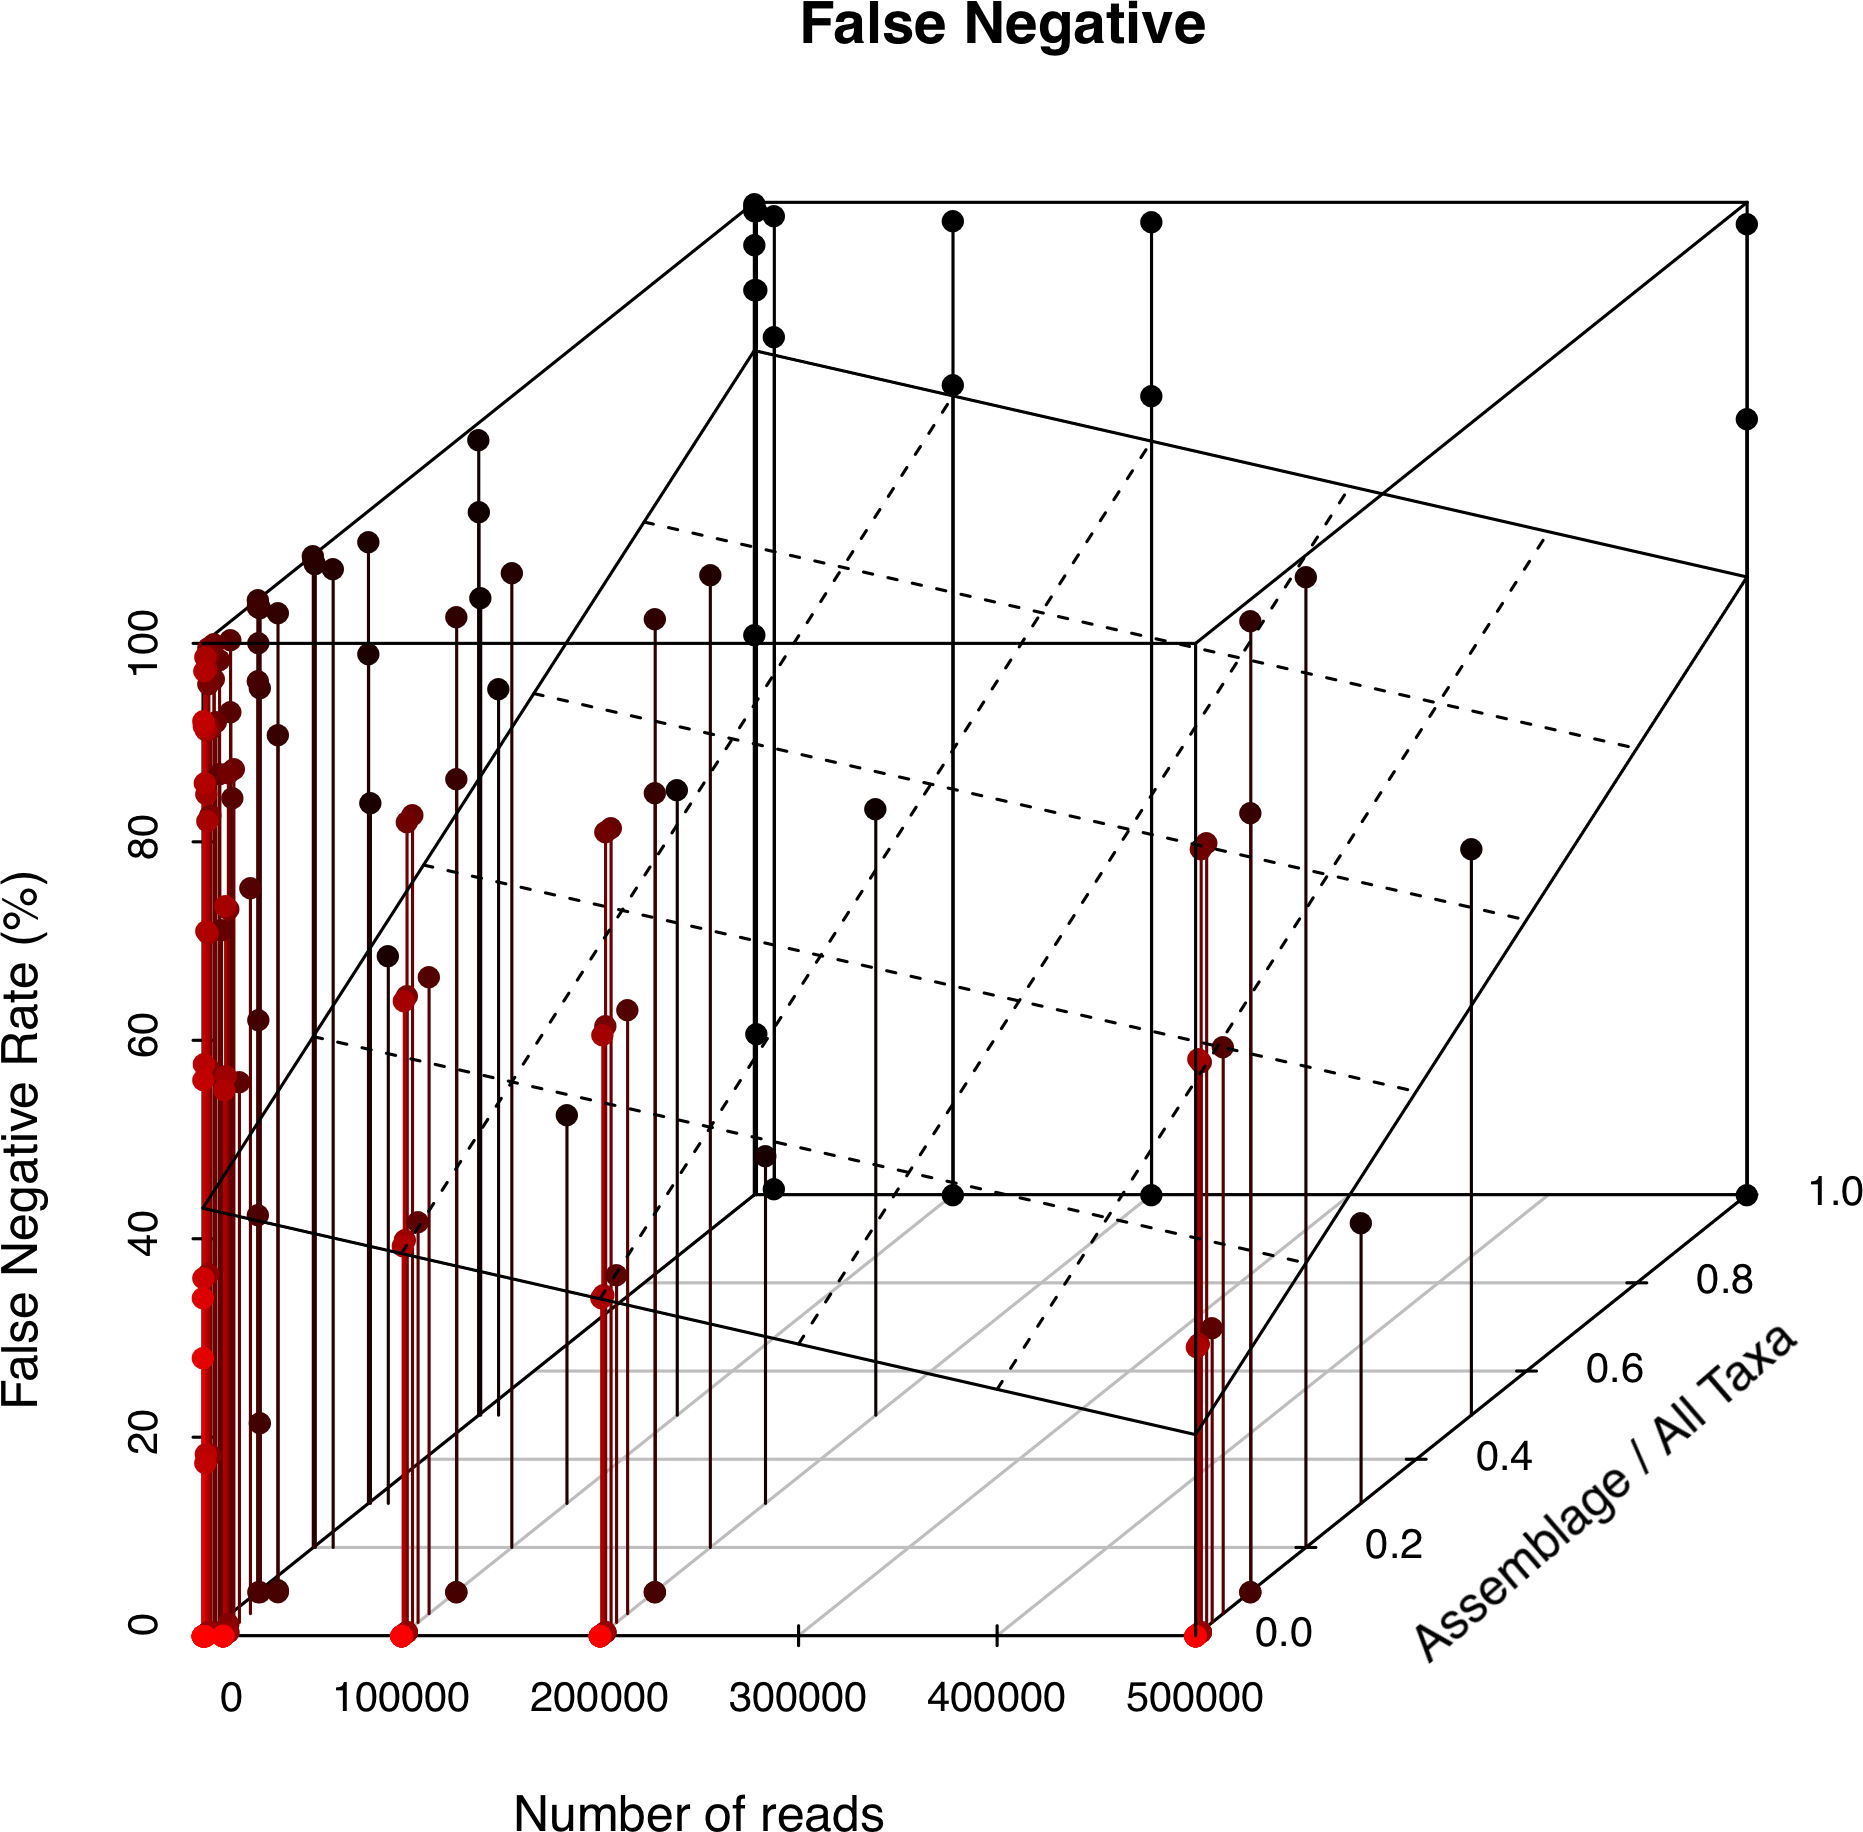
\includegraphics[width=0.45\textwidth]{../minspec/falsenegative.png}
}

&
%\quad %add desired spacing between images, e. g. ~, \quad, \qquad etc. 
%(or a blank line to force the subfigure onto a new line)

\subfloat[\sffamily{}\softwarename{minspec}-attributable false negative rate (\%) --- the percentage of \acp{OTU} not in the assemblage that generated \softwarename{blast} hits but were incorrectly removed by \softwarename{minspec}.\label{fig:minspecvalidationminspecfalsenegative}]{
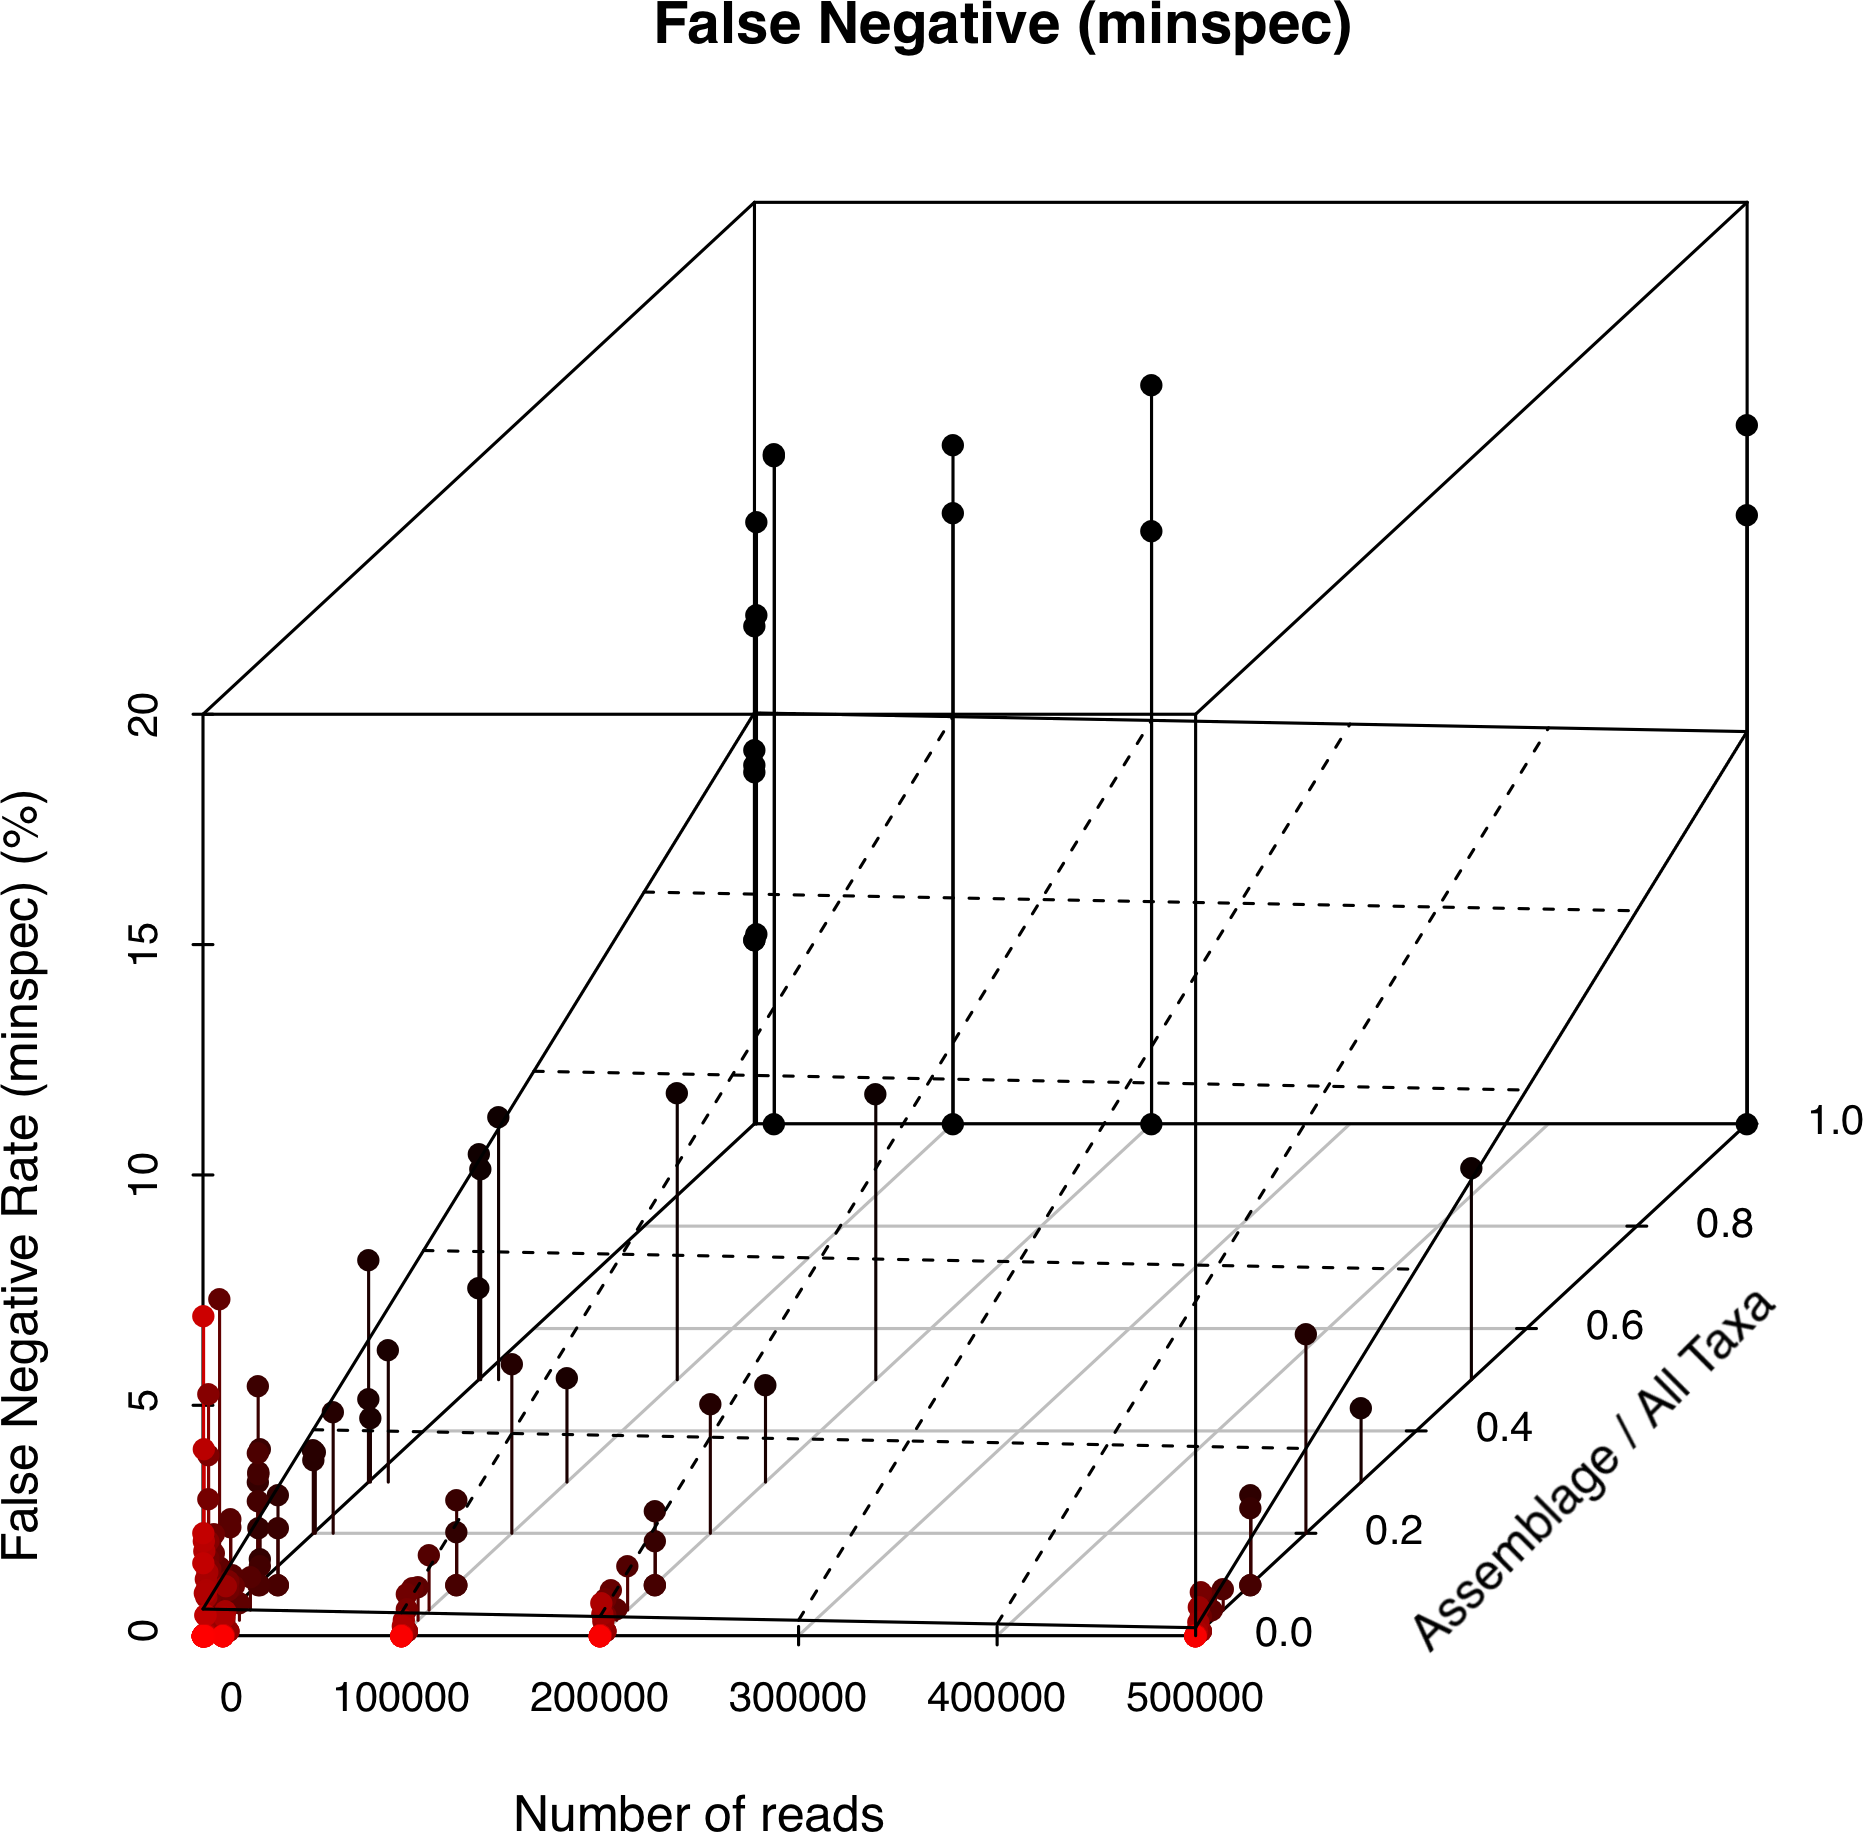
\includegraphics[width=0.45\textwidth]{../minspec/minspecfalsenegative.png}
}
\bigskip
\\
\bigskip
\\
%\quad %add desired spacing between images, e. g. ~, \quad, \qquad etc. 
%(or a blank line to force the subfigure onto a new line)

\subfloat[\sffamily{}False positive rate (\%) --- the percentage of \acp{OTU} not in the assemblage that were present in the \softwarename{blast} results following \softwarename{minspec} processing. \label{fig:minspecvalidationfalsepositive}]{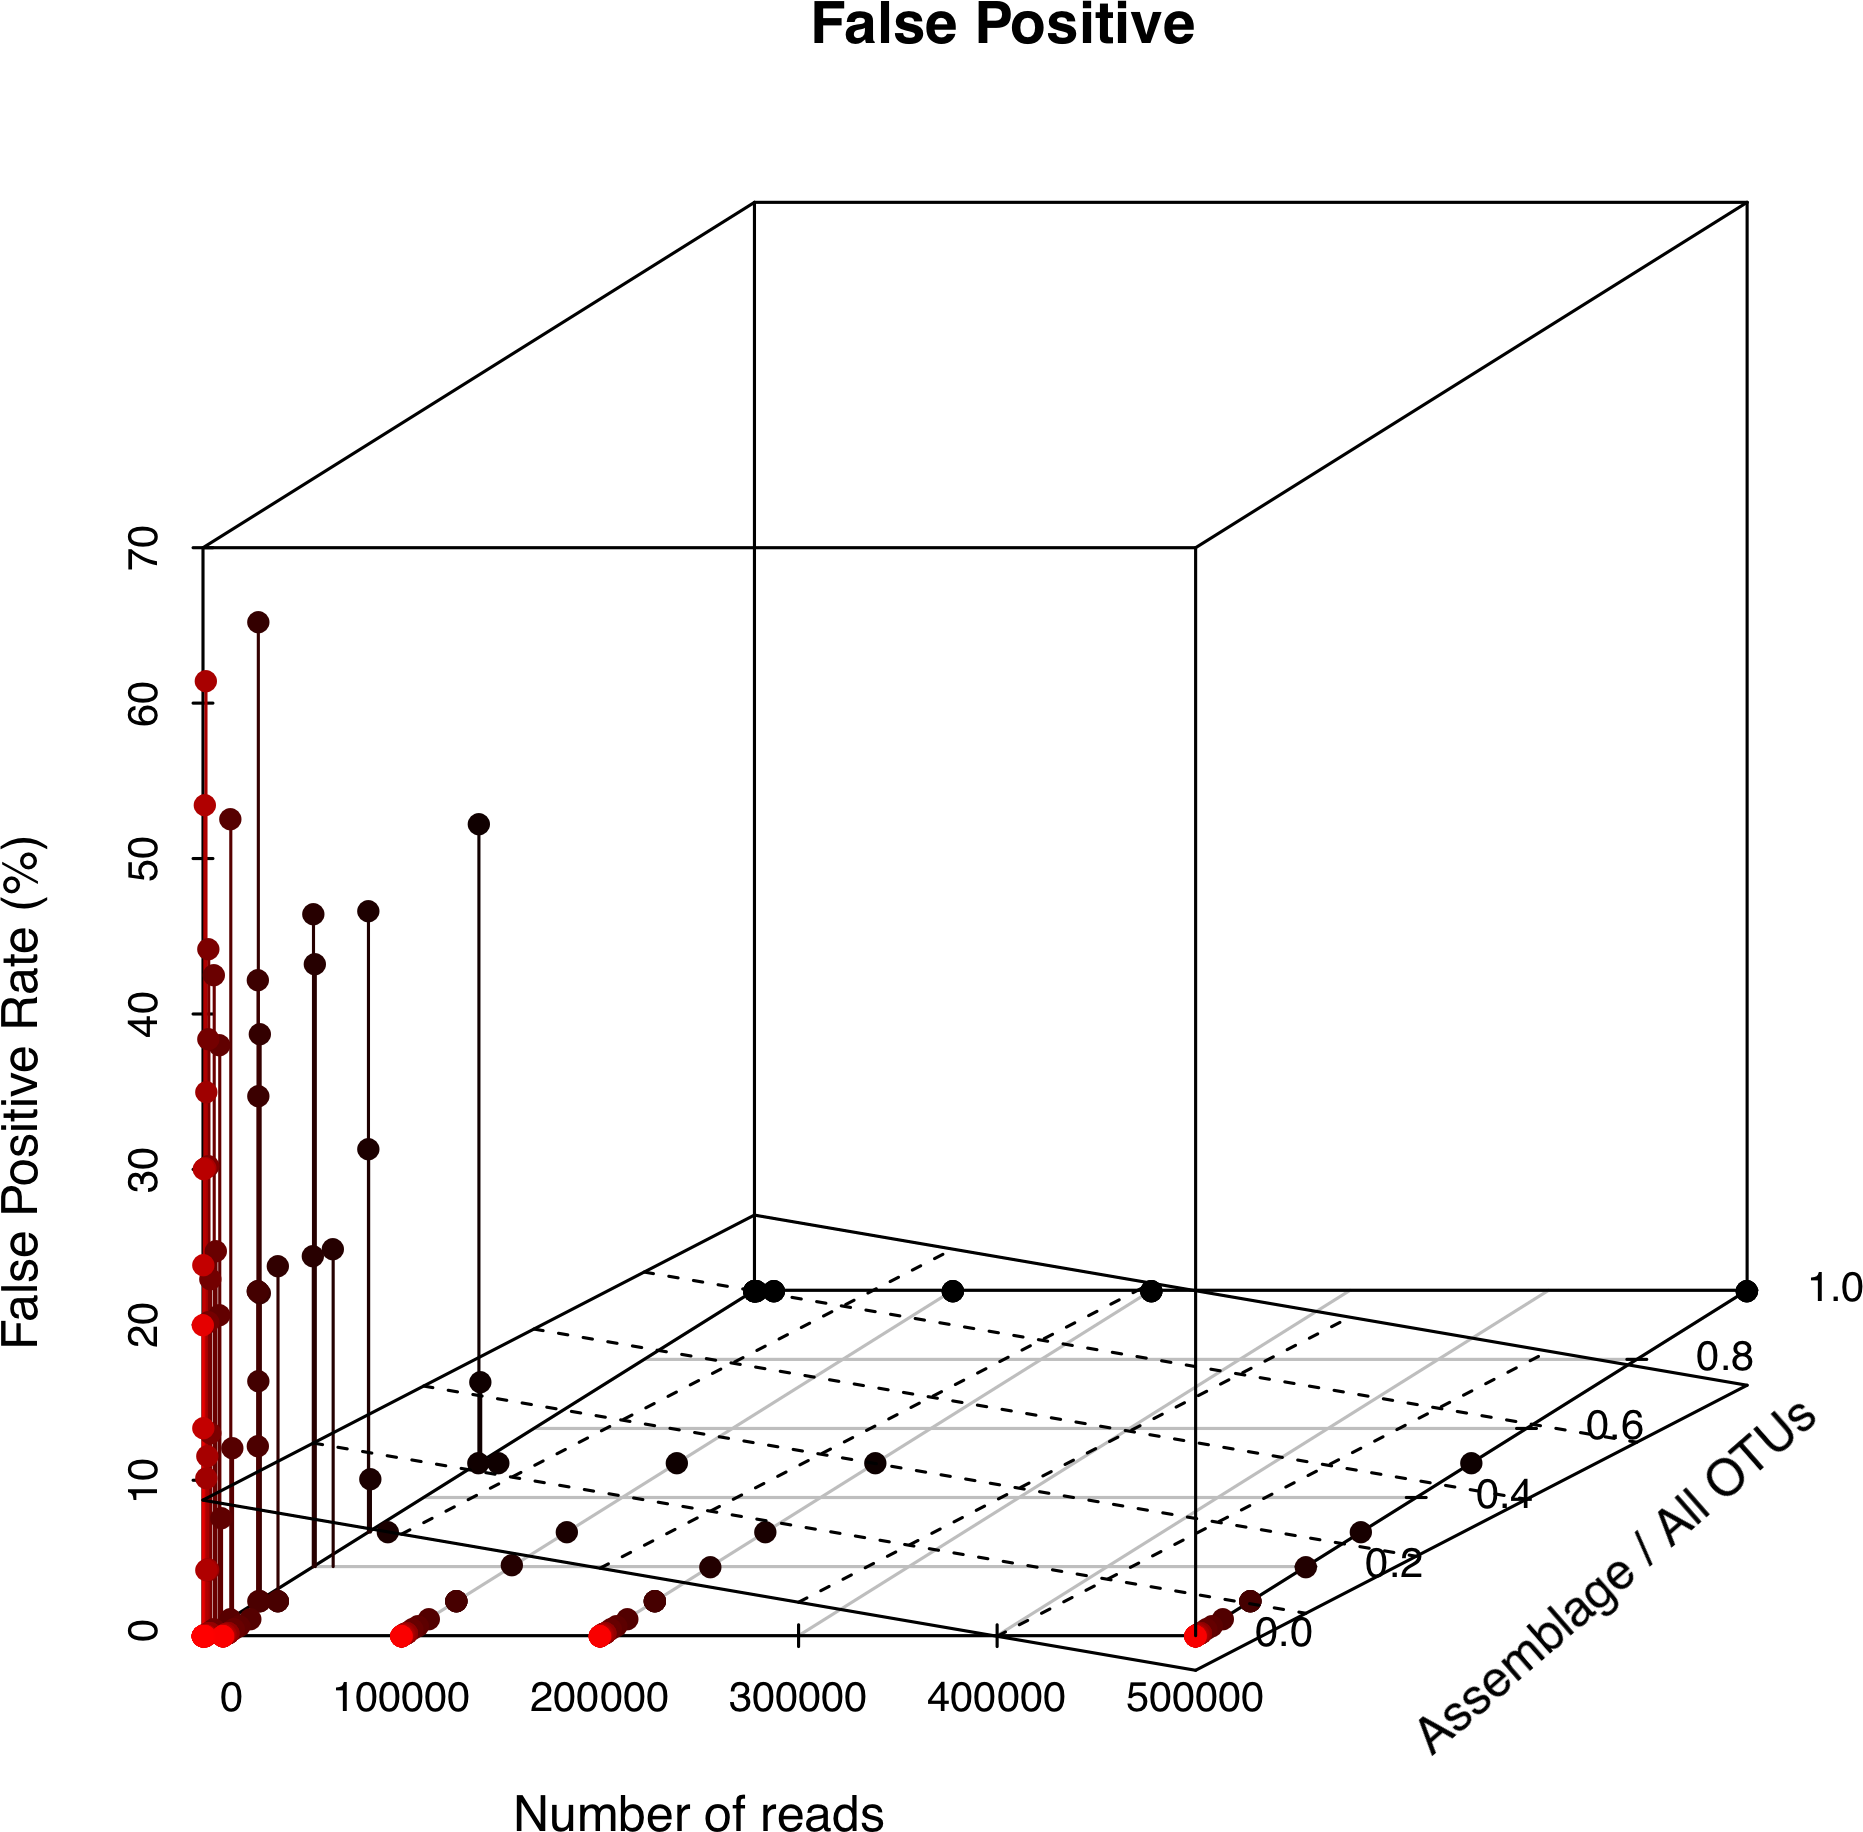
\includegraphics[width=0.45\textwidth]{../minspec/falsepositive.png}}

&
%\quad %add desired spacing between images, e. g. ~, \quad, \qquad etc. 
%(or a blank line to force the subfigure onto a new line)

\subfloat[\sffamily{}Proportion of false \acp{OTU} --- \acp{OTU} that were not part of the simulated assemblage but which generated hits due to simulated sequence identity --- that were correctly identified and removed by \softwarename{minspec}.\label{fig:minspecvalidationfalseotusaremoved}]{
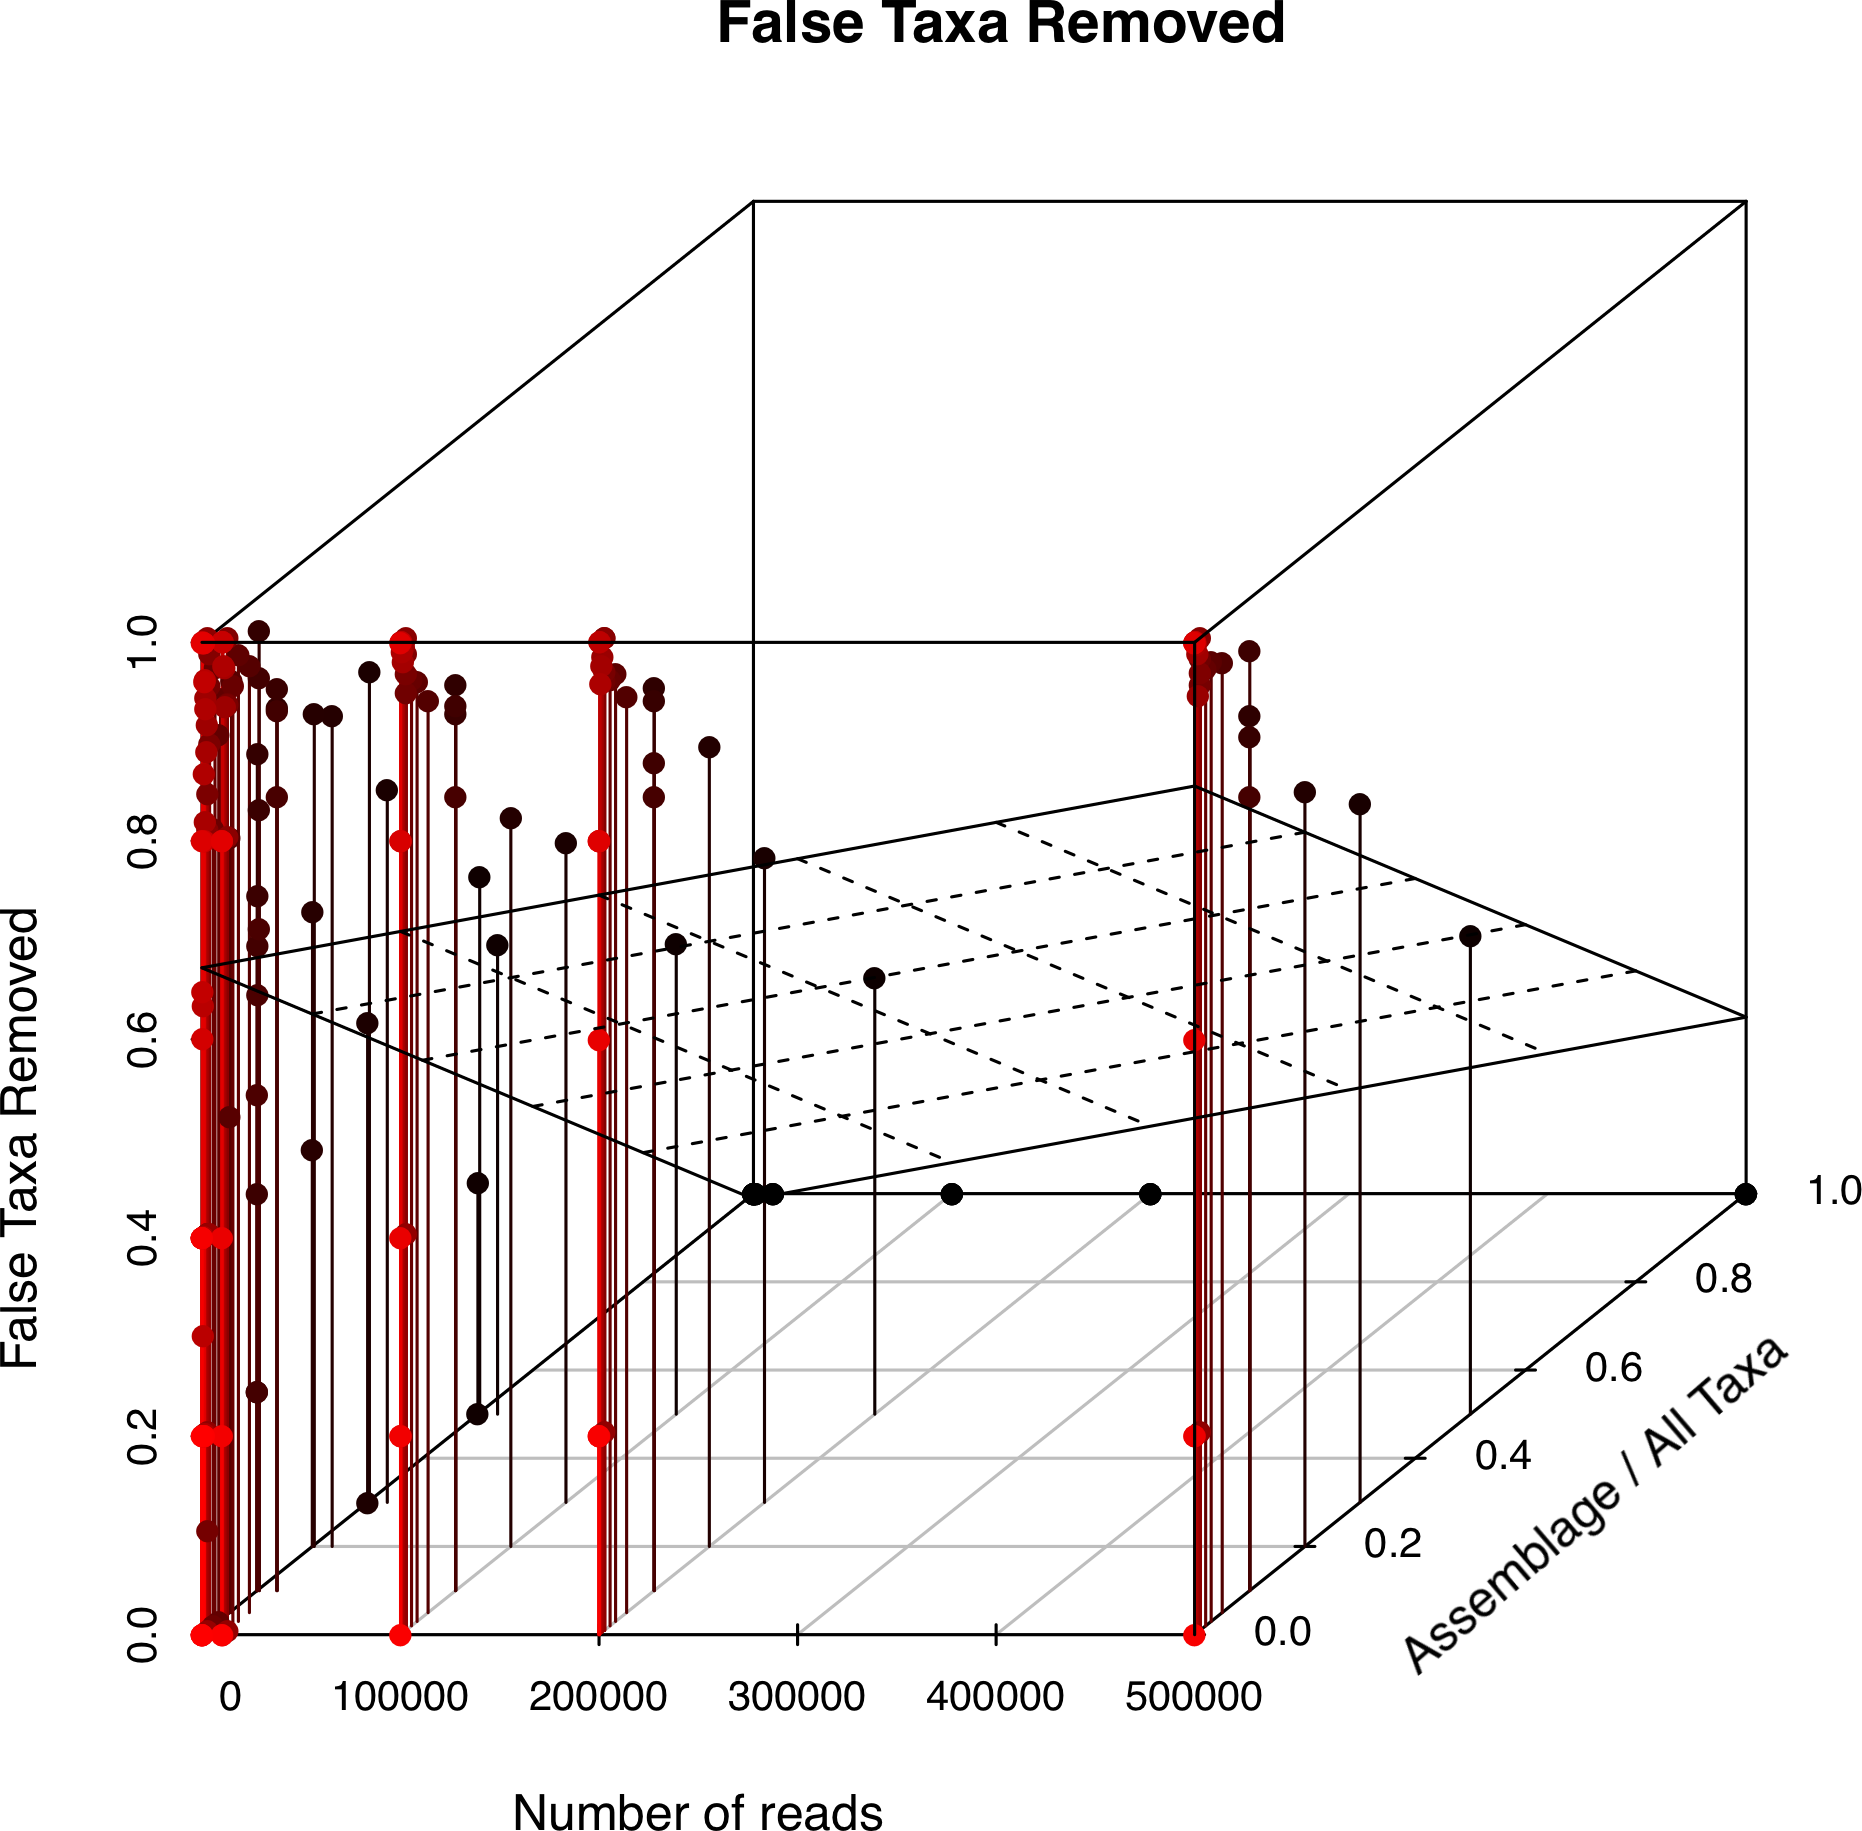
\includegraphics[width=0.45\textwidth]{../minspec/falseotusremoved.png}
}
\\

\end{tabular}

\caption[Results of \softwarename{minspec} validation]{Results of repeated trials of \softwarename{minspec} on simulated metagenomic studies with multiple permutations of parameters (number of reads, number of simulated \acp{OTU}, size of simulated assemblage).
The number of simulated \acp{OTU} and size of simulated assemblage are represented as a ratio on the z-axis (``assemblage / all \acp{OTU}'').
Each permutation was repeated five times.
A plane representing a linear regression has been overlaid on each plot to indicate the trend.
Points have been tinted to aid the perception of depth; colour is not otherwise meaningful.
}\label{fig:minspecvalidation}
\end{figure}


The false negative rate, or percentage of taxa in the assemblage which were absent from the \softwarename{blast} results following \softwarename{minspec} processing, was generally high, ranging from \textapprox{} 20\% under ideal conditions (a low assemblage / all taxa ratio, and 500,000-read metagenomic sample) to \textapprox{} 90\% in the worst case (a high assemblage / all taxa ratio and a small metagenomic sample) \figref{fig:minspecvalidationfalsenegative}.
The assemblage / all taxa ratio (hereafter referred to as ``assemblage ratio'') indicates the proportion of simulated taxa (``all taxa'') which was chosen to form the simulated assemblage.
A higher ratio means it is more likely on average that any randomly selected taxon is part of the assemblage, and thus that any individual failure to detect a taxon is incorrect.
This problem is mitigated with increasing the number of reads, as this makes it less likely that a given taxon would go undetected.
The extreme false negative rates, in some cases 100\%, represent extreme simulated scenarios (e.g.\ an assemblage of 1 taxon drawn from a pool of 100,000), and thus are unlikely to reflect real metagenomic studies.

Because the majority of false negatives are attributable to undersampling and failure of taxa to generate \softwarename{blast} hits --- properties the simulated metagenomic experiments share with real ones --- a second metric, the false negative (\softwarename{minspec}) rate, was calculated \figref{fig:minspecvalidationminspecfalsenegative}.
This is the proportion of taxa in the assemblage which generated \softwarename{blast} hits, but were incorrectly removed by \softwarename{minspec}.
This rate thus represents error attributable only to \softwarename{minspec}.
The false negative (\softwarename{minspec}) rate was generally low, ranging from \textapprox{} 0--1\% for low assemblage ratios, to \textapprox{} 15--20\% under high ratios.
Surprisingly, increasing the number of reads only slightly decreased the rate, at both low and high assemblage ratios.
This may be because \softwarename{minspec} requires only one read which has identity to a single taxon to ensure that taxon is not removed.

The false positive rate, or percentage of taxa not in the assemblage which nevertheless generated high-quality \softwarename{blast} matches that were not removed by \softwarename{minspec}, was generally \textapprox{} 0--5\% except for extremely small read sets and low assemblage ratios, where it reached as high as 60\% \figref{fig:minspecvalidationfalsepositive}.
These results reinforce the value of larger read sets, and show that once a modest metagenome size is reached (\textapprox{} 100,000 reads) very few false positives can be expected.

The proportion of false taxa removed was calculated to measure \softwarename{minspec}'s success at identifying and eliminating taxa which are not part of the sampled assemblage yet generate high-quality \softwarename{blast} matches.
This rate varied from 0--1 depending on the parameters of the assemblage \figref{fig:minspecvalidationfalsetaxaremoved}.
For simulations with a low assemblage ratio, the proportion was generally high ($> 0.6$), although there were simulated experiments with a low ratio where the proportion was low or zero.
However, in all simulations with an assemblage ratio of 1, the proportion was 0, and the regression indicated a generally inverse relationship between the ratio and the proportion of false taxa removed.
This is likely because in assemblages with a higher assemblage ratio, there are fewer false taxa to remove; in assemblages with a ratio of 1, there are none.
The high proportion of false taxa correctly identified in simulations with a low assemblage ratio is thus a good indication that \softwarename{minspec} is generally successful at identifying and removing false taxa, especially as this proportion far exceeds the false positive and false negative (\softwarename{minspec}) rates for comparable experiments.
As expected, increasing the number of reads improved \softwarename{minspec}'s accuracy.

Overall, the simulated experiments validated both the accuracy and usefulness of \softwarename{minspec} as a tool for reducing error in metagenomic studies.
It is worth noting that the assemblage ratio is not an inherent property of an assemblage, although it is limited by the assemblage's species richness.
Rather, it can be decreased, and thus the accuracy of the metagenomic experiment improved, by performing \softwarename{blast} searches against larger databases with finer taxonomic resolution.
These results thus reinforce the value of both large read sets and comprehensive reference databases in obtaining high-quality metagenomic results.

\section{Discussion}

